\section{Introduction}\label{intro}\sloppy
Images and video are the frontier of modern data management with hundreds of hours of video uploaded to YouTube every minute, the immense data generated from CCTV footage, and a possible future with autonomous driving. There has been recent interest in visual analytics (VA)~\cite{anderson2018predicate, kang2018blazeit,kang2017noscope, wu2018querying, sparks2017keystoneml}, where the visual content of the videos is analyzed.
The growing maturity of neural networks for image prediction and segmentation problems has made this an attractive and inter-discplinary field of study; bringing together systems research and large-scale machine learning.

While it is natural to connect this recent interest with prior work on multimedia databases~\cite{yoshitaka1999survey}, the recent instantiations of VA systems only loosely borrow from past architectural designs. Current types of architecture suffice since the focus has been on relatively simple analytics tasks. 
As a concrete example, consider the problem of finding all images that contain a vehicle.
One can stream videos or static images through  Mask-RCNN~\cite{he2017mask}, which is a neural network that returns a set of segmentation masks and classifications of those segmentations from a discrete set of labels (e.g., vehicle, person, cat). 
From those predictions, one can simply filter all predictions that match the desired labels.
Answering such queries is mostly bottlenecked by neural network inference.

\red{ae: at some point early should we introduce a system term like VDMS and outline the data model?}

\begin{figure}[t]
% \vspace{-5pt}
\centering
 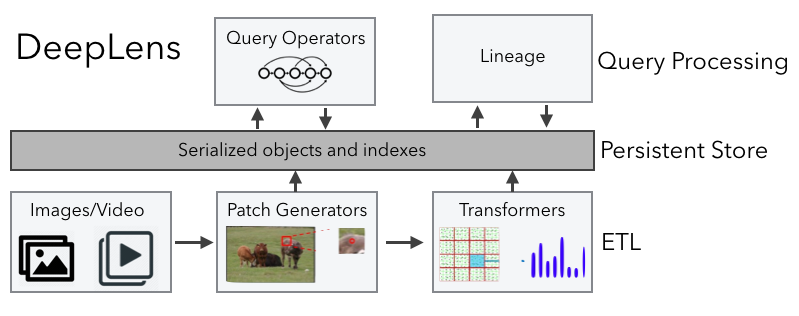
\includegraphics[width=\columnwidth]{figures/teaser.png}
 \caption{DeepLens has a dataflow-like architecture for processing visual analytics queries. All analysis is cast as relational queries on relations of image patches. Intermediate results can be materialized and indexed.  \label{teaser} }
\end{figure}

Now, consider a marginally harder query: \emph{given two videos find all vehicles that appear in both videos}.
Answering such a query is not simply a question of evaluating a predicate along each stream of images.
One has to first find all the vehicles in both videos and then match them against each other.
Efficiently answering this sort of query raises questions about physical design (should one build an index of frames with cars), query optimization (which video to scan and which index to use), and compression (can the query be answered from features instead of raw frames).
For traditional data, DBMS systems automatically handle many of these questions, and ideally, VA systems should do so as well.

This paper takes the position that a relational data model can greatly simplify the user-facing programming interface to scale VA to more complex tasks.
We revisit the idea of a multimedia database in the era of deep learning. 
This database can load corpora of images, videos and answer semantic queries about the content in these videos based on a library of computer vision algorithms that segment, annotate, and process images.
We start with a ``green field'' architectural design and built a prototype system, called \textsf{DeepLens}, which implements an ETL layer, storage layer, indexing, and query processing.
\red{ae: not clear why relational is the right data model at this point, what parts of it are being borrowed?} 



\textsf{DeepLens} is designed similarly to a dataflow query processing system~\cite{graefe1994volcano}. There are access methods which point to iterators over images derived from a filesystem or sampled from a video stream. The image dataflow is passed into a  \textbf{patch generator} that turns the image into a set of patches either by fixed or semantic criteria.\red{Adam: What are the fixed criteria?} Associated with each patch is a key-value dictionary. \red{Adam: Is the dictionary mapping from a property of the patch to its value, e.g. the property being a size of the patch and the value being its width and height, or a property being a source image and the value being a path or id of the source image?} The patches are then fed into a composition of \textbf{transformers} that featurize, compress, or otherwise store detected properties of the patches into the dictionary. Over tuples of transformed patches, users can build a directed computation graph with \textbf{operators} (e.g., select, join).
The patch abstraction defines a closed-algebra where the input is a patch and the output is a patch for all of the operators.
Furthermore, tuple-level lineage is automatically maintained by the system allowing any downstream patch to be associated with its base data.
Any of the intermediate results can be \textbf{materialized} and can be stored in clustered and unclustered formats. \red{What are the clustered and unclastered formats? Maybe a citation could be added here?}
Furthermore, indexes can be built on any materialized data, either the key-value attributes or the image data.
We show that this model is sufficient to describe a large number of visual analytics tasks.


We present initial experimental results on these components to elicit some of the key open research challenges. To summarize our key lessons learned:

\vspace{0.5em}

\noindent \emph{Lesson 1. Image data is unstructured data. } Semantics from images have to be first extracted with computer vision algorithms before structured queries can be executed. We found that many VA queries can be formulated as different types of joins and filters on the outputs of these algorithms and relating those results back to the base data. \textsf{DeepLens} includes an ETL component in which different types of computer vision algorithms can run and maintains provenance to the original image or video. This ETL component also modulates the accuracy of the system where image resolution and frame sampling rates can be controlled.      

\vspace{0.5em}

\noindent \emph{Lesson 2. True multimedia queries vs. easy queries. }
Queries that have to relate structured outputs to pixel data in the images are challenging to process. This is because we have to mix different physical design paradigms to answer such queries. Structured outputs such as label predictions can be indexed with hash tables and B+ Trees. However, pixel data is multi-dimensional and is best indexed with spatial indexes. Sometimes that pixel data is position (x,y pixel values) and can easily be stored in an R-Tree or similar structures. In other cases, the pixel data is a featurized fingerprint (e.g., reverse image search) and requires a structure optimized for higher dimensional dense vector data like a KD-Tree. Deciding which indexes to create is very workload specific.


\vspace{0.5em}

\noindent \emph{Lesson 3. Almost all processes are compute-limited. }
Image processing algorithms are very compute intensive. This differs from classical DBMS models where IO costs are dominant. 
Many classical indexing, query processing, and query optimization frameworks are designed with IO-limited models in mind.
In a compute-limited world, there is a new space of optimization that can be explored.
In \textsf{DeepLens}, we present a data-skipping framework that skips processing after a page has been loaded into memory. For example, suppose we have an expensive neural-network classifier UDF \texttt{isRedCar(image)}, images that do not have a sufficient number of red pixels can be discarded upfront before evaluating the expensive predicate. We also discuss the implications of compute-limited processes on query optimization and physical design.









